% Pancake networks
% Author: Anthony Labarre <http://homepages.ulb.ac.be/~alabarre/home.html>
\documentclass{minimal}

% Tikz
\usepackage{tikz}
\usepackage{verbatim}

\begin{comment}
:Title: Pancake network

The pancake network of order n has the set of all permutations of {1,2,...,n}
as vertex set and has an edge between any two vertices such that the
corresponding permutations can be obtained from one another by reversing the
order of the first k elements of the permutation (e.g. (1 2 3 4) will be connected to
(2 1 3 4), (3 2 1 4) and (4 3 2 1), but not to (1 4 3 2)). This drawing shows
the pancake network of order 4.

\end{comment}

\newcommand{\LD}{\langle}
\newcommand{\RD}{\rangle}

\begin{document}

\begin{center}
 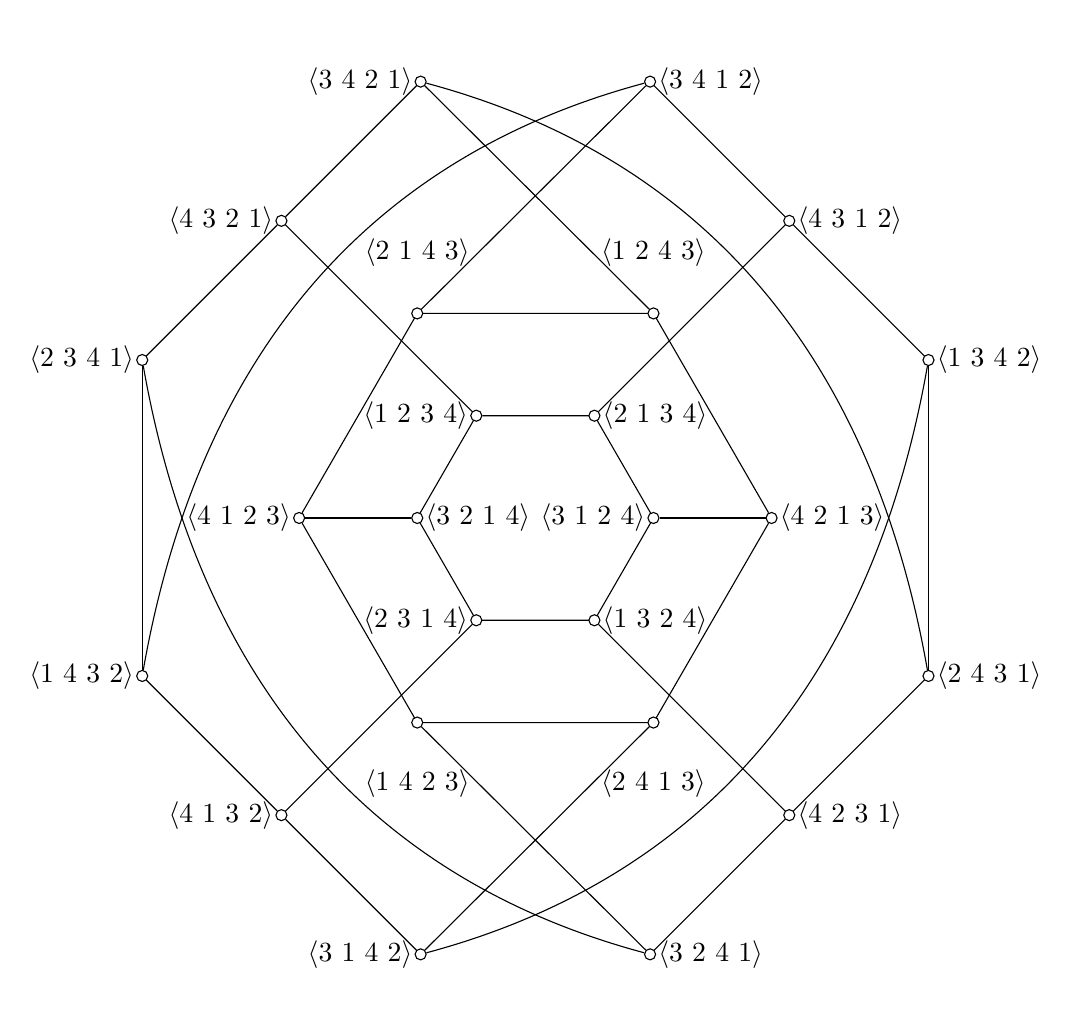
\begin{tikzpicture}
    \tikzstyle{every node}=[draw,circle,fill=white,minimum size=4pt,
                            inner sep=0pt]

    % First, draw a ``bug'', which is a regular hexagon with ``legs'' attached
    % to each vertex
    % This is the hexagon:
    \draw (0,0) node (1234) [label=left:$\LD 1\ 2\ 3\ 4\RD$] {}
        -- ++(240:1.5cm) node (3214) [label=right:$\LD 3\ 2\ 1\ 4\RD$] {}
        -- ++(300:1.5cm) node (2314) [label=left:$\LD 2\ 3\ 1\ 4\RD$] {}
        -- ++(0:1.5cm) node (1324) [label=right:$\LD 1\ 3\ 2\ 4\RD$] {}
        -- ++(60:1.5cm) node (3124) [label=left:$\LD 3\ 1\ 2\ 4\RD$] {}
        -- ++(120:1.5cm) node (2134) [label=right:$\LD 2\ 1\ 3\ 4\RD$] {}
        -- (1234);

    % And these are the legs:
    \draw (1234) -- ++(135:3.5cm) node (4321) [label=left:$\LD 4\ 3\ 2\ 1\RD$] {};
    \draw (2134) -- ++( 45:3.5cm) node (4312) [label=right:$\LD 4\ 3\ 1\ 2\RD$] {};
    \draw (1324) -- ++(-45:3.5cm) node (4231) [label=right:$\LD 4\ 2\ 3\ 1\RD$] {};
    \draw (2314) -- ++(225:3.5cm) node (4132) [label=left:$\LD 4\ 1\ 3\ 2\RD$] {};
    \draw (3124) -- ++(0:1.5cm) node (4213) [label=right:$\LD 4\ 2\ 1\ 3\RD$] {};
    \draw (3214) -- ++(180:1.5cm) node (4123) [label=left:$\LD 4\ 1\ 2\ 3\RD$] {};

    % Build outer regular hexagon
    \draw (4213)
        -- ++(120:3.0cm) node (1243) [label=above:$\LD 1\ 2\ 4\ 3\RD$] {}
        -- ++(180:3.0cm) node (2143) [label=above:$\LD 2\ 1\ 4\ 3\RD$] {}
        -- (4123)
        -- ++(-60:3.0cm) node (1423) [label=below:$\LD 1\ 4\ 2\ 3\RD$] {}
        -- ++(0:3.0cm) node (2413) [label=below:$\LD 2\ 4\ 1\ 3\RD$] {}
        -- (4213);

    % Now ``decorate'' the other legs a bit
    \draw (4321) -- ++(45:2.5cm) node (3421) [label=left:$\LD 3\ 4\ 2\ 1\RD$] {};
    \draw (4132) -- ++(-45:2.5cm) node (3142) [label=left:$\LD 3\ 1\ 4\ 2\RD$] {};
    \draw (4231) -- ++(225:2.5cm) node (3241) [label=right:$\LD 3\ 2\ 4\ 1\RD$] {};
    \draw (4312) -- ++(135:2.5cm) node (3412) [label=right:$\LD 3\ 4\ 1\ 2\RD$] {};

    % Add missing nodes
    \draw (4231) -- ++(45:2.5cm) node (2431) [label=right:$\LD 2\ 4\ 3\ 1\RD$] {};
    \draw (4312) -- ++(-45:2.5cm) node (1342) [label=right:$\LD 1\ 3\ 4\ 2\RD$] {};
    \draw (4321) -- ++(225:2.5cm) node (2341) [label=left:$\LD 2\ 3\ 4\ 1\RD$] {};
    \draw (4132) -- ++(135:2.5cm) node (1432) [label=left:$\LD 1\ 4\ 3\ 2\RD$] {};

    % Add missing ``straight'' edges
    \draw (3421) -- (1243);
    \draw (2143) -- (3412);
    \draw (1423) -- (3241);
    \draw (3142) -- (2413);
    \draw (1432) -- (2341);
    \draw (1342) -- (2431);

    % Add missing ``curved'' edges
    \draw (2341) to [out=-80,in=165] (3241);
    \draw (3142) to [out=15,in=260] (1342);
    \draw (1432) to [out=80,in=195] (3412);
    \draw (2431) to [out=100,in=-15] (3421);

\end{tikzpicture}
\end{center}

\end{document}
